% 如果你想添加多个附录,你可以这样做:

% \ThesisAppendix
% \chapter{附录标题1}

% \section{占位符1}

% 随机文本1

% \chapter{附录标题2}
% 附录内容2

% 如果你只想添加一个附录,你可以这样做:

\ThesisSingleAppendix
% \chapter{附录标题}

\section{占位符2}

随机文本2

\begin{figure}[htb]
    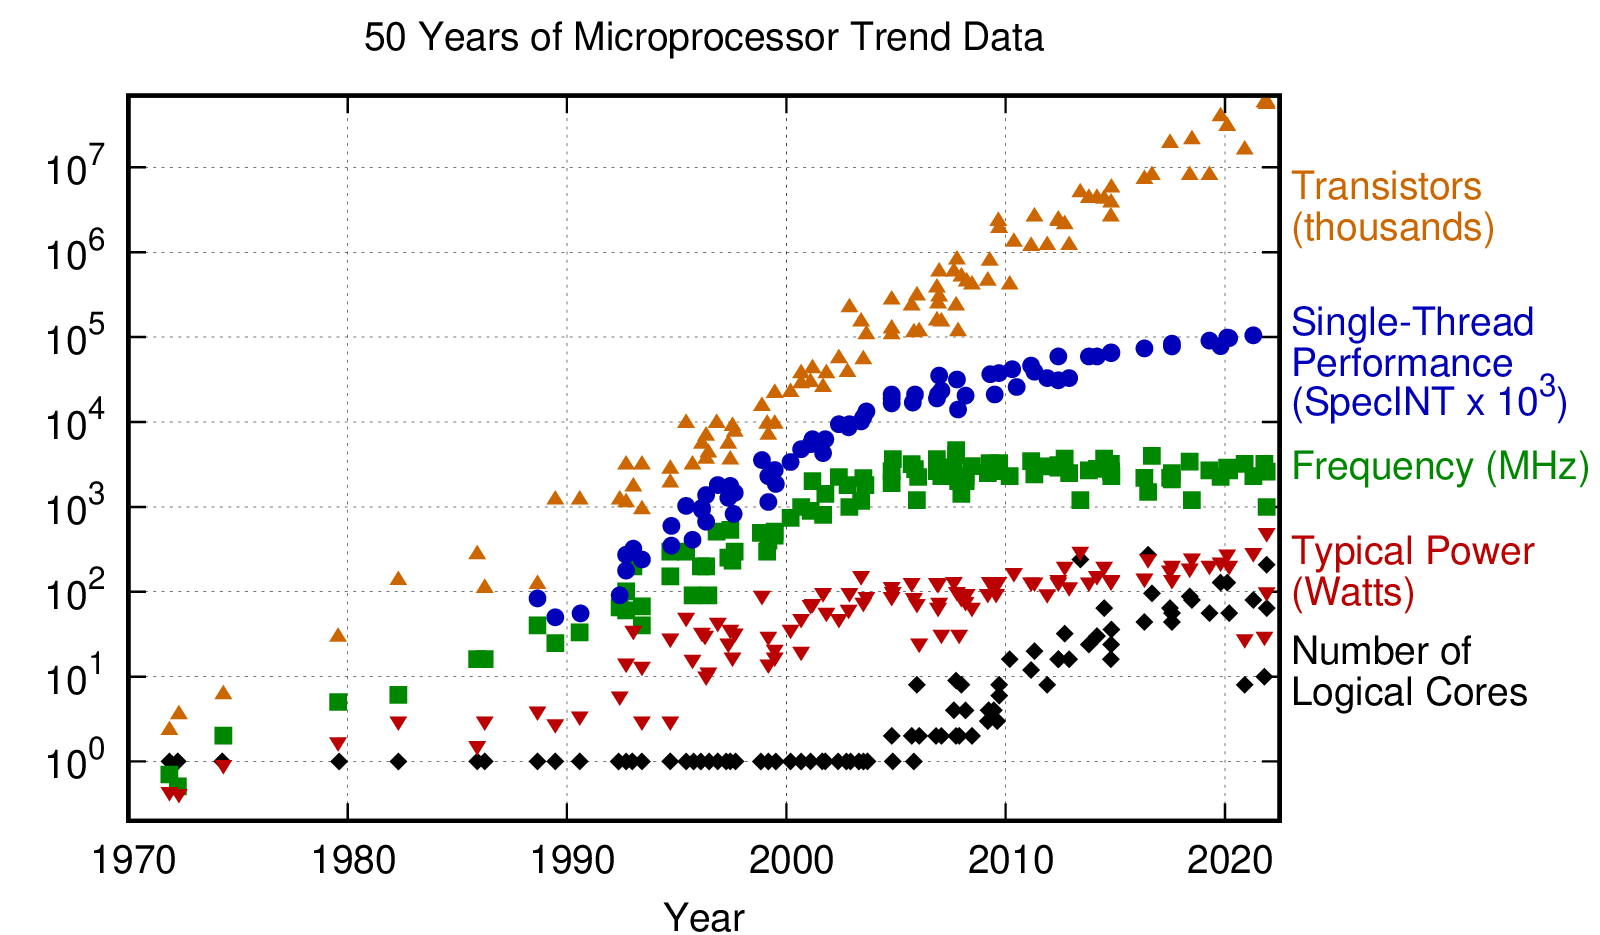
\includegraphics[width=0.8 \textwidth]{50-years-processor-trend.png}
    \caption[处理器发展]{近50年微处理器发展趋势} % 中括号中内容为插图索引中显示内容,可在题注内容过长时使用
    \label{fig:processor-trend}
\end{figure}

图片引用示例:\cref{fig:processor-trend}。
% 在这两个例子中,\chapter命令用于添加一个新的附录章节。你可以在\chapter命令后面写上你的附录内容。